%Befehle: 
% \newpage - Neue Seite
% \section{Ueberschrift} - Kapitelueberschrift "Ueberschrift"
% \ subsection {Ueberschrfit} - Ueberschrift eines Abschnittes
% Papierformat
\documentclass[a4paper, 12pt]{article}
% Silbentrennung Deutsch
\usepackage[ngerman]{babel} 
% UTF8
\usepackage[utf8]{inputenc}
% Import von Grafiken
\usepackage{graphicx}
% URLs
\usepackage{url}
% BibLaTeX
\usepackage[backend=bibtex,style=alphabetic,sorting=debug]{biblatex}
\usepackage[strings]{underscore}
\DeclareFieldFormat{labelalpha}{\thefield{entrykey}}
\DeclareFieldFormat{extraalpha}{}
\addbibresource{./Dokumentation/Quellen}{}
\usepackage{float}
% Anfang Dokument
\begin{document}
\thispagestyle{empty}
% Deckblatt
	%Thema
	% Lässt Zeilen leer
\begin{verbatim}



\end{verbatim}
\begin{center}
	\Large{Extraktion großer Geometrien}
\end{center}
\begin{center}
\textbf{\Large{Dokumentation}}
\end{center}
	% Lässt Zeilen leer
\begin{verbatim}





\end{verbatim}
	% HTW Infos
\begin{center}
	\Large{Hochschule für Technik und Wirtschaft Berlin}
\end{center}
\begin{center}
	\Large{Fachbereich 4  Informatik, Kommunikation und Wirtschaft}
\end{center}
\begin{center}
	\Large{Studiengang Angewandte Informatik}
\end{center}
	% Füllt Text bis Seiten Ende
\vspace*{\fill}
	% Author und Datum
\begin{flushleft}

\begin{tabular}{lll}
\textbf{Eingereicht von:} & & Meron Nagy\flq{}nagy.meron@gmail.com\frq{}\\
& & Eduard Andreev \flq{}s0558738@htw-berlin.de\frq{}\\
& & \\
\textbf{Eingereicht am:} & & 28.05.2018\\
& & \\
\textbf{Betreuer:} & & Herr Prof. Dr.Ing. Thomas Schwotzer
\end{tabular}
\end{flushleft}

	\newpage
% Inhaltsverzeichnis
\tableofcontents
	\newpage
% Einleitung
\section{Einleitung}
\subsection{Rahmen}
Mit OHDM entstand im Rahmen der Lehre ein System, das ähnlich wie OSM Kartendaten bereit
stellt. Im Gegensatz zu OSM werden aber nicht nur aktuelle Karten sondern auch historische
angeboten. Ein wesentliche Quelle von Daten für OHDM ist OSM. OSM sammelt aktuelle Daten.
Diese Daten archivieren wir in OHDM. Was heute aktuell ist, ist morgen Geschichte. \\
	\newline
Die Daten in OSM kommen aber regelmäßig in einer sehr feinen Granularitäten. Oft werden
Straßenzüge in vielen einzelnen Teilgeomtrien beschrieben. Das ergibt sich allein aus der Art der
Datenerhebung: Menschen laufen durch mit GPS Receivern durch die Gebiete und vermessen die
Landschaft. Diese GPS-Tracks sind die Basis der OSM (und damit auch OHDM) Karten.
Bundesstraßen, Landesgrenzen und Flüsse sind gute Beispiele für große geometrische Objekte, die
durch eine Vielzahl von Einzelgeometrien erfasst wurden. In OSM werden diese großen Geometrien
oft durch Relationen beschrieben. Relationen beschreiben ein Objekt (z.B. eine Landesgrenze)
indem sie dem Objekt einen Namen geben (z.B. „Grenze der BRD“) und ordnen diesem Objekte Geometrien zu.
	\subsection{Aufgabe}
Ziel ist es, Verfahren zu entwickeln, um Einzelgeometrien zu einer großen Geometrie zusammen zu
fassen. Es soll mit den Landesgrenzen angefangen werden. Die Daten liegen derzeit als eine Menge
von Linen vor, die durch Relationen zusammen gefasst sind. Diese Linien sind zu einem Polygon
zusammen zu fassen.\\
	\newline
Das klingt soweit trivial und wäre es auch, wenn die OSM Freiwilligen nicht große Freiheitsgrade
in der Beschreibung der Geometrien haben. Manchmal entstehen Lücken, die sich aber
algorithmisch schließen lassen. Es kann teilweise auch ein Datenbankproblem werden. Man möge
sich die Landesgrenzen der USA vorstellen – die OSM Karten der USA sind sehr feingranular.
Damit ist die Landesgrenze eine Summe einer enormen Menge an einzelnen Teil-Geometrien\cite{rahmen}.
	\newpage
\section{Deployment}
Das Programm wird über ein Konsolenmenü gesteuert.
Wenn noch keine login.properties Datei existiert, müssen Datenbank (Bsp.: postgresql://ohm.f4.htw-berlin.de:5432/ohdm_public),  Nutzername und Passwort der OHDM Datenbank eingegeben werden.
Jetzt können über Menüpunkt 1 die Linestrings heruntergeladen werden. Dafür müssen Schema und Tabellenname angegeben werden. 
Nachdem die Linestrings heruntergeladen wurden können die Polygone über den Menüpunkt 2 zusammengesetzt werden. Hierfür müssen auch Schema und Zieltabelle angegeben werden.
Das Ergebnis ist eine Geojsondatei die im Rootverzeichnis des Programms gespeichert wird. Diese kann dann zur Ansicht bei mapshaper.org hochgeladen werden.
% Hauptteil
\section{Grundlagen}
\subsection{PostGIS}
PostGIS ist eine PostgreSQL Erweiterung für Geodaten. Die Erweiterung fügt neue Befehle für die Arbeit mit Geoobjekten hinzu\cite{pgis}.
\subsection{WGS 84 / Pseudo-Mercator}
Pseudo-Mercator ist eine Projektionsvariante zum erzeugen von digitalen Karten\cite{wgs}. 
\subsection{Definitionen}
\subsubsection{Point}
 Ein räumlicher Punkt repräsentiert einen Ort auf der Erde. In unserem Fall wird ein Punkt in Längen- und Breitengraden angegeben.\\
\subsubsection{Linestring}
 Ein Linestring beschreibt den Weg zwischen Punkten. Er besteht aus einer geordneten Reihe von Punkten. Der erste Punkt des Linestrings wird als Head definiert und der letzte als Tail.\\
\subsubsection{Polygon}
 Ein Polygon beschreibt eine Fläche. Es wird aus einem geschlossenen Linestring gebildet. Ein Linestring ist geschlossen wenn Head und Tail identisch sind\cite{geome}.

	\newpage
\section{Wesentliche eigene Arbeit}
\subsection{Anforderungen }
\subsubsection{Musskriterien}
Es soll eine algorithmische Lösung gefunden werden, um aus einzelnen Linestrings von Landesgrenzen, Polygone zu bilden. \\
Der Algorithmuss soll dabei so allgemeingültig wie möglich sein, um ihn später auch für andere Geometrien einsetzen zu können.\\
\subsubsection{Wunschkriterien}
Es soll ein Javaprogramm entwickelt werden, welches aus den OHDM Daten eine neue Tabelle mit Polygonen der einzelnen Landesgrenzen erzeugt.\\
\subsubsection{Abgrenzungskriterien}
Im Verlauf dieses Projektes wird das Javaprogramm nur mit Landesgrenzen verwendbar sein.\\
\subsection{Extraktion der Daten aus der OHDM Datenbank}
Die GeoDaten werden mithilfe von Java und dem PostgreSQLJDBC Treiber entweder für die Weiterverarbeitung herruntergeladen und in Java Objekte umgewandelt oder im JSON Format zwischengespeichert\cite{jdbc}.
\subsection{Visualisierung der Geodaten für Testzwecke}
Die im vorherigen Kapitel gewonnen Daten müssen umformatiert werden.
Die formartierte GeoJSON Datei wird dann mit Hilfe von http://geojson.io/ oder http://mapshaper.org/ visualisiert.
Wäh­rend geojson.io über eine Karte im Hintergrund verfügt, besitzt mapshaper.org nur einen weißen Hintergrund, kann dafür aber mit größeren Daten schneller arbeiten und benötigt die GoeJson Daten nicht in einer Featurecollection.
\subsection{Visualisierung der Geodaten für Testzwecke}
Ideen: Algorithmus der Kreisbildet und ausreißer entfernt: Startpunkt: beliebige landesgrenze die im Namen "Deutschland" oder ähnliches enthält
Algorithmus zuerst in Java realisieren
Prüfen ob anfang und ende des Linestrings 2x in der GeoJSON datei vorkommen, wenn ja speichern
\section{Herrausforderungen}
Nach genauerem Betrachten der Daten haben sich einige Herrausforderungen herrausgebildet.\\
Zum einen weisen einige der Linien Lücken auf, zum anderen besitzen andere kein "sinnvolles" Ende und scheinen ins Nirgenswo zu verlaufen. Wieder andere verlaufen an der selben stelle mehrfach. \\
Außerdem muss eine sinnvolle Lösung gefunden werden, wie der Algorithmus auf verschiedene Ereignisse, wie das auftreten mehrerer möglicher Wege reagiert.\\
Eine weitere Herrausvorderung stellt die Arbeit in Java mit großen Datenmengen dar.\\
\subsection{Vorüberlegungen und Herangehensweise}
Um diese Herrausvorderungen zu bewältigen wurde ein Schichtenmodell entwickelt.\\
Jede Schicht soll einzelne Herrausforderungen bearbeiten um somit das große Problem iterativ verkleinern bis sich am Ende eine, den Anforderungen entsprechende, Lösung ergibt.\\
\subsection{Algorithmusbeschreibung: allgemein}
Im allgemeinen werden die Daten Schritt für Schritt vereinfacht. Somit entstehen weniger einzelne Daten, welche iteriert werden müssen und die zu verarbeitenden Datensätze werden auf das nötigste reduziert. Einzelne, eindeutig zusammengehörige Linestrings werden z.B. zu großen Linestrings verbunden. Einzelne Punkte eines Linestrings, die nicht für weitere Berechnungen benötigt werden, werden zunächst aussortiert und doppelte Linien entfernt.\\
Jetzt kann damit begonnen werden, Linien zu suchen, welche eindeutig zu einem Polygon gehören und diese zu verbinden.\\
\subsection{Beschreibung: detailliert}
Zuerst werden die Linestrings der Grenzen aus der Datenbank herruntergeladen. In diesem Fall ist das die Tabelle Admin_boundary_2.
Die einzelnen Linestrings werden hier als kleine Linien (siehe Abb. 1) bezeichnet. Sie haben oft keine Bezeichnung grenzen aber meist an weiteren Linestrings an, sprich Tail einer Linie, ist meist der Head einer anderen.
\begin{figure}[H]
  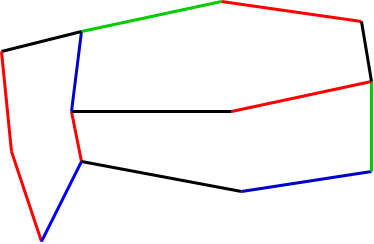
\includegraphics[scale=0.7]{Dokumentation/kleineLinien.png}
  \caption{kleine Linien: Ausgangssituation.}
  \label{fig:kleineLinien}
\end{figure}
Diese Eigenschaft wird verwendet, um aus den einzelnen Linestrings, größere zu erstellen. Begonnen bei der Ersten Linie wird geprüft ob sich ein Head oder Tail findet, der mit dem Head, der zu prüfenden Linie, identlisch ist. Falls dieser Fall eintritt und genau eine weitere Linie gefunden wird, werden die Linien zu einer verbunden.  Es entstehen die hier genannten großen Linien.
\begin{figure}[H]
  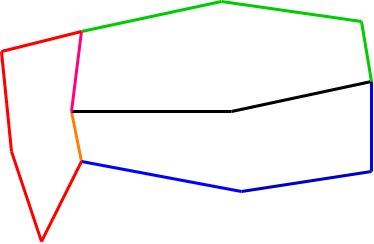
\includegraphics[scale=0.7]{Dokumentation/grosseLinien.png}
  \caption{goße Linien.}
  \label{fig:grosseLinien}
\end{figure}
Im nächsten Schritt werden doppelt auftretende Punkte und Linien gelöscht. Und die großen Linien werden in die Datenbank hochgeladen. Über einen Regexbefehl in der Datenbank, werden nur die ersten beiden und letzten beiden Punkte einer Linie als Linestring herruntergeladen, da die Zwischenwerte für die weitere Berechnung irrelevant sind. Damit die Linien aber wieder zugeordnet werden können, bekommen sie einen Idex.
\begin{figure}[H]
  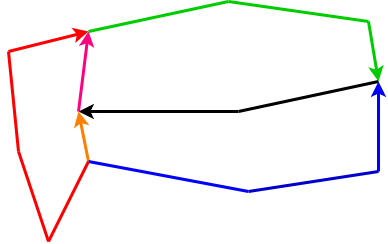
\includegraphics[scale=0.7]{Dokumentation/RichtungHeadTail.png}
  \caption{RichtungHeadTail.}
  \label{fig:RichtungHeadTail}
\end{figure}
Eine Linie ist eine Sortierte Menge von Punkten mit einem Anfang(Head)und einem Ende(Tail) sind....damit...müssen die Linien gedreht werden. +++
\begin{figure}[H]
  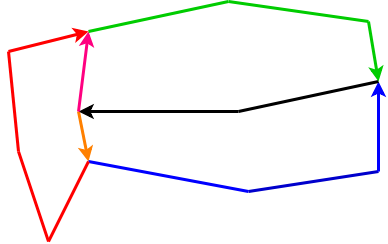
\includegraphics[scale=0.7]{Dokumentation/Linie_Drehen.png}
  \caption{Linie_Drehen.}
  \label{fig:Linie_Drehen}
\end{figure}
Um ein  einzelnes Polygon nach einem anderen zu bilden, werden die Winkel zwischen der aktuell betrachteten Linie(schwarz) und allen angrenzenden Linien gemessen und der kleinste Winkel bestimmt. Damit bekommt der Algorithmus eine feste Laufrichtung zugewiesen. 
\begin{figure}[H]
  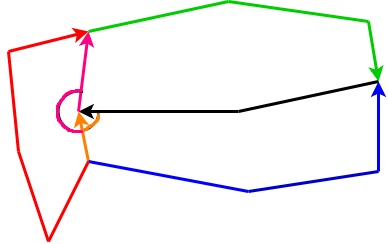
\includegraphics[scale=0.7]{Dokumentation/1.png}
  \caption{Winkel1.}
  \label{fig:Winkel1}
\end{figure}
 Dieser Prozess wird solange ausgeführt bis der eigene Ursprung gefunden wurde oder es keine Abzweigungen mehr gibt. 
\begin{figure}[H]
  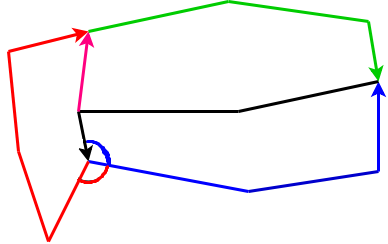
\includegraphics[scale=0.7]{Dokumentation/2.png}
  \caption{Winkel2.}
  \label{fig:Winkel2}
\end{figure}
Tritt der erste Fall auf, wird der Linestring zu einem Polygon verbunden.
\begin{figure}[H]
  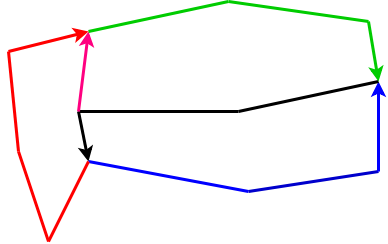
\includegraphics[scale=0.7]{Dokumentation/Polygon_bilden1.png}
  \caption{Polygon_bilden.}
  \label{fig:Polygon_bilden}
\end{figure}

\begin{figure}[H]
  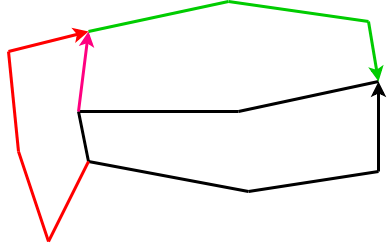
\includegraphics[scale=0.7]{Dokumentation/Polygon.png}
  \caption{Polygon_bilden.}
  \label{fig:Polygon_bilden}
\end{figure}
 Tritt der zweite Fall auf, wurde eine Lücke gefunden. Um eine Lücke zu schließen wird die kleinste Distanz zum nächstgelegen Anfang/Ende einer Linie gesucht.
\begin{figure}[H]
  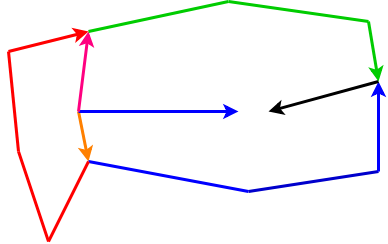
\includegraphics[scale=0.7]{Dokumentation/FehlendeLinie.png}
  \caption{FehlendeLinie.}
  \label{fig:FehlendeLinie}
\end{figure}
In diese Lücke wird eine neue Linie eingefügt um den Linestring zu einem Polygon zu schließen.
\begin{figure}[H]
  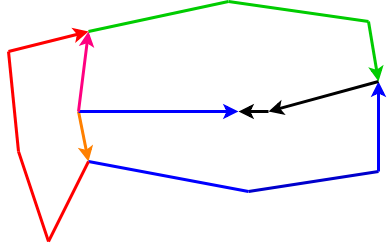
\includegraphics[scale=0.7]{Dokumentation/ZwischenLinie.png}
  \caption{ZwischenLinie.}
  \label{fig:ZwischenLinie}
\end{figure}
Abschließend werden die Polygone in die Datenbank geladen.
	\newpage
% Fazit
\section{Fazit}
Die beschriebenen Anforderungen konnten weitesgehend erfüllt werden. Testversuche haben gezeigt, dass zu einem großen Teil Sinnvolle Ergebnisse entstehen. Da es nicht leicht ist für sehr spezielle Probleme sehr allgemeingültige Lösungen zu finden und sich die Fehlersuche in der Masse an Daten, als sehr Zeitaufwendig herrausgestellt hat, war es in der gegeben Zeit nicht möglich alle aufgetretenen Fehler zu beheben.


	\newpage
% Quellen mit BibTeX https://de.sharelatex.com/learn/Bibliography_management_with_bibtex
\section{Literaturverzeichnis}
\setlength{\emergencystretch}{3em}
\printbibliography
% Ende Dokument
\end{document}